\subsection{Quality adjusted life years}
\label{sec:model_development_qalys}

\subsubsection{Health related quality-of-life measures}
\label{sec:model_development_qalys_hrqol}
In general, HRQoL measures summarize population health by a single 
preference-based index measure. A HRQoL measure is a suitable measure of QALY. 
There are several widely-used generic HRQoL indexes, each involving a standard descriptive system: a 
multidimensional measure of health states and a corresponding scoring system to translate the descriptive 
system into a single index \citep{fryback2007us}. The scoring system is developed based on a community survey 
of preference valuation of health states in the descriptive system, using utility valuation methods like time 
trade-offs or a standard gamble. 

\subsubsection{Health related quality-of-life in MEPS}
\label{sec:model_development_qalys_eq5d}
Because the health states measures in the HRS and FEM do not match the health 
states defined in any of the currently available HRQoL indexes, we used MEPS to 
create a crosswalk file for HRQoL index calculation.  MEPS collects information 
on health care cost and utilization, demographics, functional status, and medical 
conditions. Since the year 2000, it initiated a self-administered questionnaire 
for two sets of instruments: SF-12 and EQ-5D. 

Seven of the twelve SF-12 questions can be used to generate another HRQoL index: 
SF-6D. However, the scoring system for SF-6D was derived from a UK sample 
\citep{brazier2004estimation} and a significant proportion of the MEPS sample 
did not give valid answer for at least one of the seven questions. Therfore, we 
decided to calculate EQ-5D index score as the HRQoL measure for FEM. 

The EQ-5D instrument includes 5 questions about the extent of problems in 
mobility, self-care, daily activities, pain, and anxiety/depression. The scoring 
system for EQ-5D was first developed by \citet{dolan1997modeling} using a UK 
sample. Later, a scoring system based on a US sample was generated 
\citep{shaw2005us}. In MEPS 2001, there are 8,301 respondents aged 51 and over. 
Of those respondents, 7,439 gave valid answers for all of the five EQ-5D 
questions. We calculated EQ-5D scores for these respondents using the scoring 
algorithm based on a US sample \citep{shaw2005us}. The distribution of EQ-5D 
index scores among these respondents is shown in Figure 
\ref{fig:meps2001_age51p_eq5d_hist}.

\begin{figure}[h]
\centering
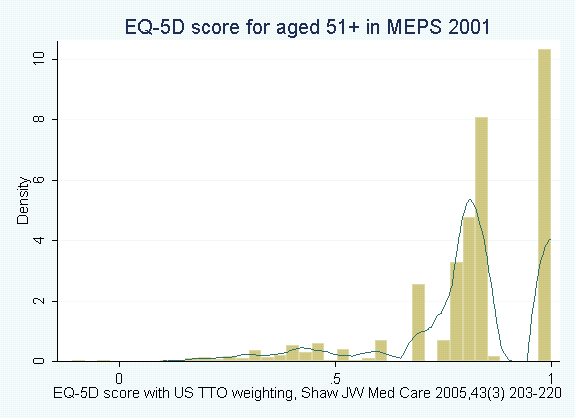
\includegraphics[scale=0.8]{./img/meps2001_age51p_eq5d_hist.png}
\caption{Distribution of EQ-5D index scores for ages 51+ in 2001 MEPS}
\label{fig:meps2001_age51p_eq5d_hist} 
\end{figure}

\subsubsection{MEPS-HRS Crosswalk development}
\label{sec:model_development_qalys_crosswalk}
The functional status measure in FEM is based on the HRS. It is a categorical 
variable including the following mutually exclusive categories: healthy, any IADL 
limitation (no ADL limitations), 1-2 ADL limitations, and 3 or more ADL limitations. 
Unfortunately the measures of IADL and ADL limitations in MEPS are quite different. 
HRS asks questions like ``Do you have any difficulty in $\ldots$'', while MEPS asks 
questions like ``Does $\ldots$help or supervision in $\ldots$.'' As Table 
\ref{tab:meps_hrs_adl_iadl_prevalence} shows, the prevalence of 
IADL limitations is relatively similar between the two surveys, while the 
prevalence of ADL limitations is much higher in HRS, relative to MEPS. This is 
reasonable since not all who have difficulty in ADLs receive help or supervision. 

In order to compute EQ-5D index scores using functional status in the FEM, we needed
a set of functional status measures that is comparable across MEPS and HRS (the host 
dataset for FEM).  We explored several options for deriving such a measure.  Ultimately,
we constructed two measures. One measure indicates physical function limitation 
while the other measure indicates IADL limitation. 

In MEPS, physical function 
limitation indicates that at least one of the following is true: 1) receiving help 
or supervision with bathing, dressing or walking around the house; 2) being limited 
in work/housework; 3) having difficulty walking, climbing stairs, grasping objects, 
reaching overhead, lifting, bending or stooping, or standing for long periods of time; 
or 4) having difficulty in hearing or vision. In HRS, physical function limitation indicates 
that at least one of the following is 
true: 1) having any difficulty in bathing/dressing/eating/walking across the room/getting 
out of bed; 2) limited in work/housework; or 3) limited in any other activities.

In MEPS, IADL limitation indicates receiving help or supervision using the telephone, 
paying bills, taking medications, preparing light meals, doing laundry, or going shopping.
In HRS, IADL limitation indicates having difficulty in any IADL such as using the phone, managing 
money, or taking medications. 

The prevalence of our two constructed measures among ages 51 and older in MEPS (2001) and HRS (1998) is 
shown in Table \ref{tab:meps_hrs_physlim_iadl_prevalence}. The prevalences are quite similar across the two surveys. 

Using MEPS 2001 data, we next use ordinary least squares to model the derived EQ-5D score as a function of six 
chronic conditions -- which are available both in HRS and MEPS, our two constructed measures of functional status, 
and an interaction term of the two measures of functional status. Three different models were considered. 
Estimation results are presented in Models I-III in Table \ref{tab:meps_eq5d_model_est}. We also show the estimation results of using only 
IADL/ADL limitation as covariates, and using only the six chronic conditions as covariates, as Models IV and V in 
Table \ref{tab:meps_eq5d_model_est}. Model II was used as the crosswalk described 
in Section \ref{sec:estimation_qalys} to calculate EQ-5D score for non-nursing 
home residents aged 51 and over in HRS 1998.



